%-----------------------------------------------------------------------------------------
\clearpage
\section{Implementation}
%-----------------------------------------------------------------------------------------

\subsection{Tooling}
Implementing a distributed neural network is too large a task to be undertaken
from scratch. Therefore its necessary to used existing tools, to make the
development viable in the time given. This is difficult as not many languages
lend themselves to both distributed systems and neural networks.

To ensure high performance the project could be implemented in C++. While C++ is
often very performant and also has low level bindings for ML libraries such as
TensorFlow. However even the creator of the language sees the need to improve
its ability to improve its distributed performance. \cite{stroustrupInterview}

Python has great tooling for neural networking, such as TensorFlow
\cite{abadi2016tensorflow}, and PyTorch \cite{paszke2019pytorch}. Moreover it
has great support for numerical computing with NumPy \cite{harrisNumpy2020}.
These are performant too, by calling C functions or creating code which is
optimised to run on GPUs to parallelise computation. However due to the Global
Interpreter Lock (GIL) python is infamously bad at concurrency, while its
distributed tooling is implemented in native python code, which lack of speed
and could bottleneck the performance gained from using NumPy and TensorFlow.

Ultimately I decided to use Elixir as the programming language of
implementation. This is because Elixir was designed for developing highly
concurrent distributed systems. It does this by having a uniquely brilliant
concurrency model. As opposed to OOP languages where 'everything is an object'
in Elixir 'everything is a process'. This means the default way of writing the
language enables it to be concurrent and scalable. Elixir also has the ability
to communicate with other Elixir programs over the network using its own
application protocol on top of TCP/IP. Meaning its as easy to communicate with
local processes on your own machine as processes on another machine running an
Elixir program. Its also been used by artificial intelligence researchers before
as the process concurrency models effortlessly lends itself to modelling
neurons. \cite{sherNeuroevolutionThroughErlang} Using Elixirs native float and
arithmetic implementation would be slower than a C++ or a NumPy implementation,
luckily there is a stable package which supports matrix calculations even faster
than those in NumPy called Matrex. \cite{matrex}

The only drawback of using Elixir is at the time of development it didn't have a
strong machine learning library, which means implementing the mathematics of the
neural network myself. While this was a sizeable amount of work to do, it had
the benefit that I didn't to wrestle with an opinionated API such as TensorFlow,
I could create my own API to meet my ends.

\subsection{Neural Network Implementation}
In order to create a distributed neural network. I first needed to create a
basic feed forward network that could operate on a single machine. This network
doesn't need to be fully featured, its just a means to make an objective
comparison between RingTMP and a generic parameter server. Therefore only 2
types of layers were implemented, the hidden layer and the output layer. The
hidden layer is a generic dense layer similar to the kind you would find in any
other neural network library. The output layer performs similarly to the hidden
layer with the key difference that its always the final layer in a network and
outputs the activations as probabilities. Within this section I will explain in
more detail how the neural network was implemented from scratch and the
mathematics behind its function.

% creating a network should go here first
\subsubsection{Initialisation}
Neural networks are composed of layers, while conceptually layers are
composed of neurons, they're practically implemented with two components. A
weights matrix and a bias vector. As I have already mentioned in this network
there are two types of layers, hidden layers and output layers. We need to label
each layer with its type, so we know how to perform forward and
backpropagation. Therefore we can describe a layer as the tuple:
\begin{lstlisting}[numbers=none,frame=none]
    {layer_type, weights, bias}
\end{lstlisting}

Placing several of these tuples in a list creates a network:
\begin{lstlisting}[numbers=none,frame=none]
  network = [{:hidden_layer, weights_1, bias_1},
                {:hidden_layer, weights_2, bias_2},
                {:output_layer, weights_3, bias_3}]
\end{lstlisting}

The weights and biases have different dimensions depending on the layers input
size and output size. A layer might take an activations vector with a size of
\(m\) and output a size of \(n\). The layer would hold a \(n \times m\) matrix
and the dimensions of the bias would be \(n \times 1\). The output size of one
layer must be the input size of the next layer. Initialising the biases is
simple, as biases have the function of an intercept in a linear equation, they
can be initialised to 0. The trivial code is below:
\begin{lstlisting}
  defp initialise_bias(col) do
    Matrex.zeros(col, 1)
  end
\end{lstlisting} 
Weights are more complex. Each layer is initialised with random values from a
uniform distribution, the shape of the uniform distribution is dependant upon
the size of the input and output layers of the neural network. The type of
initialisation used is dependant upon the activation function used.

In the hidden layer the ReLU function is used, common wisdom first established
in this paper \cite{he2015delving} states that for the fastest convergence He
initialisation should be used. He initialisation is done by sampling random
values from a normal distribution with a mean of 0 and a variance of \( 2/N \)
where \(N\) represents the number of input values to a layer.

For the output layer, the softmax function is used. The best initialisation
method in this case is using Xavier
initialisation. \cite{glorot2010understanding} This also takes random samples
from a normal distribution with a mean of 0 but has the variance of \( 1/N \)
where \(N\) is \( (inputSize + outputSize) / 2 \).

However in practice training the model often failed with He initialisations.
This was because of what is known as the 'Dying ReLU Problem'. Which is when the
elements of a z vector are negative, the ReLU activation function
will return a zero meaning no learning is taking place. Once a neuron becomes
dead its unlikely it will be revived as the function is piecewise and provides
no slope for recovery such as a Leaky ReLU or a sigmoid function. To remedy this
I trialed many distributions, settling on a mean of 0.5 with a variance of 0.25.
While this is more simplistic, and may impact training times, its far more
likely for the network to not be dead on arrival because of the initialisation
parameters. This is part of the code which initialises the matrices in the layers:
\begin{lstlisting}
  defp random_val(_x, {n, :he, seed_state, acc}) do
    {val, new_state} = :rand.normal_s(0, 2 / col, seed_state)
    {col, :he, new_state, [val | acc]}
  end

  defp random_val(_x, {n, :pos, seed_state, acc}) do
    {val, new_state} = :rand.normal_s(0.5, 0.25, seed_state)
    {n, :pos, new_state, [val | acc]}
  end

  defp random_val(_x, {n, :xavier, seed_state, acc}) do
    {val, new_state} = :rand.normal_s(0, 1 / col, seed_state)
    {col, :xavier, new_state, [val | acc]}
  end
\end{lstlisting}
You can find the wider context for this code snippet in code listing in the Appendix 1. ~\ref{network_initialisation} 


\subsubsection{Forward Propagation}
In forward propagation we give an input vector and an output vector is returned.
In order for that to happen the input vector is passed through each layer, each
time being transformed by the weights, bias and activation function of that
layer. The input to the network could be measurements describing a flower (like
in the setosa dataset), the output layer could describe which species. More
broadly put, the input described the features, and the output predicts the
categories to which those features belong.

On a layer level forward propagation is performed by taking the input vector
multiplying it with the weights matrix, after which you add the bias and apply
the activation function. The output of this is then passed to the next layer, or
if its the last layer, output as the network prediction result. The generic
mathematics of a forward function is described below in this linear equation
where  \(X\) is the input matrix, \(W\) is the weights, \(B\) is the bias,
\(activationFunc(x)\) is the activation function and finally \(A\) is the output
activation:
\begin{equation}
    \begin{aligned}
        X = \begin{bmatrix}
            x_{1} \\
            x_{2} \\
            x_{3}
        \end{bmatrix} \, \, \, \, \, \, \,
        W &= \begin{bmatrix}
            w_{11} & w_{12} & w_{13} \\
            w_{21} & w_{22} & w_{23}
        \end{bmatrix} \, \, \, \, \, \, \,
        B = \begin{bmatrix}
            b_{1} \\
            b_{2}
        \end{bmatrix} \\[10pt]
        A &= activationFunc( W^{T}X + B )
    \end{aligned}
\end{equation}

In my implementation there are only two layer types. Hidden layers and output
layers. The only difference between these two layers is the activation function
that they use. Hidden layers use the ReLU activation function which is a simple
piecewise non-linear function described as such:
\begin{equation}
    relu(z) = max(0,z)
\end{equation}
This function has become the de facto application function in dense hidden
layers since its debut in 2011. \cite{glorot2011deep}. In Elixir the forward
action in the hidden layer is implemented like so: \footnote{The pipe operator
\lstinline{|>} transforms the function \lstinline{val_a |> a_function(val_b)}
into \lstinline{a_function(val_a, val_b)}}
\begin{lstlisting}
defmodule HiddenLayer
  def forward(previous_activation, weights, bias) do
    weights |> Matrex.transpose()
    |> Matrex.dot(previous_activation)
    |> Matrex.add(bias)
    |> relu()
  end

  defp relu(z_vector) do
    z_vector|> Matrex.apply(
        fn value, _index -> if value > 0, do: value, else: 0 end
    )
  end

  ...
\end{lstlisting}

The output layer uses a more complex activation function, the softmax function,
which transforms its inputs into probabilities. The sum of these probabilities
is always 1. This is the softmax function, where \(z\) is a \(i \times 1\)
vector:
\begin{equation}
    softmax(z)_{i} = \frac{e^{z_{i}}}{\sum_{j=1}^{n} e^{z_{j}}}
\end{equation}

This function is implemented the categorical output layer like so:
\begin{lstlisting}
defmodule CategoricalOutputLayer do
  def forward(previous_activation, weights, bias) do
      weights |> Matrex.transpose()
      |> Matrex.dot(previous_activation)
      |> Matrex.add(bias)
      |> softmax()
  end

  defp softmax(z_vector) do
      stabilised_vec = Matrex.subtract(z_vector, Matrex.max(z_vector))
      exp = Matrex.apply(stabilised_vec, :exp)
      Matrex.divide(exp, Matrex.sum(exp))
  end

  ...
\end{lstlisting}

% show forward propagation function across the networks
Propagating forward through the layers happens by using the output of one
layer as the input to the next, performing a slightly different forward action
depending on the layer:

PUT IN APPENDIX
\begin{lstlisting}
defmodule FeedForwardNetwork.Forward do
  def forward(network, input_vector) do
    Enum.reduce(network, input_vector, fn layer, acc -> forward_layer(layer, acc) end)
  end

  defp forward_layer({:hidden_layer, weights, bias}, prev_activation) do
    {_z_vec, activation} = HiddenLayer.forward(prev_activation, weights, bias, [])
    activation
  end

  defp forward_layer({:output_layer, weights, bias}, prev_activation) do
    CategoricalOutputLayer.forward(prev_activation, weights, bias, [])
  end

  ...
\end{lstlisting}

\subsubsection{Cost Function}
A neural network is trained by using examples of correct classifications based
on given data. The data is input into the network, and the network attempts to
label the data correctly. The networks prediction is compared to the correct
classification using a cost function, this gives a single value representation
describing how close or far the network was to the correct classification. A
perfect classification will result in a score of 0, the more wrong the network
prediction is the larger the cost produced by the cost function. The cost 
function used in this network is categorical cross entropy, which allows for
multi class classification. It takes two inputs, an output vector \(y\) of the network
(its prediction), and the one hot encoded vector \(t\) of the target classification:
\begin{equation}
    cost(t, y) = - \sum_{i}^{C} t_{i}log(y_{i})
\end{equation}

This implementation is similar, but removed redundant computation in the cases
where \(t_{i} = 0\) the cost will always be 0. Here we also catch situations
where the activation underflows to 0, which would result in a math error as
\(log(0)\) is undefined. For the full code example see the code listing
~\ref{cost_function} in the appendix.
\begin{lstlisting}
defmodule CategoricalOutputLayer
  def loss(activation, target_activation) do
    target_position = get_target_category(target_activation)

    activation
    |> Matrex.at(target_position, 1)
    |> (fn x ->
          if x == 0.0, do: 100, else: -:math.log(x) end
        end).()
  end

  ...
\end{lstlisting}


\subsubsection{Back Propagation}
The result of the cost function represents the error within the network,
backpropagation adjusts the weights and biases to minimise the loss within the
network. Meaning that if the same input was given to the network again after
backpropagation, the output would be closer to the target, than before
backpropagation had occurred. The changes to the weights and bias of each layer
can be calculated by using the chain rule, to discover the relationship between
the weights and biases with respect to the loss.

To calculate the change in weights and biases in the output layer, we first need
to find the derivative of the cost function w.r.t the network output and the
derivative of the softmax function w.r.t \(z\).

\begin{equation}
    \begin{aligned}
        c &= - \sum_{i}^{c} t_{i}log(a_{i}) \\
        \frac{\partial c}{\partial a} &= - \sum_{i}^{c} \frac{t_{i}}{a_{i}}
    \end{aligned}
\end{equation}

Finding the derivative of the softmax is a little more complex:
\begin{equation}
    \begin{aligned}
        &       &   a_{j} &= \frac{e^{z_{j}}}{\sum_{k=1}^{N} e^{z_{k}}} \\
        &\text{applying quotient rule (for brevity} \sum = \sum_{k=1}^{N} e^{z_{k}} \text{)}   &   \frac{\partial a_{i}}{\partial z_{j}} &= \frac{e^{z_{i}} \sum - e^{z_{j}}e^{z_{i}}}{\sum^{2}}\\[2em]
        &\text{if } i=j \text{ then it can be factorised}     &   \frac{\partial a_{i}}{\partial z_{j}} &= \frac{e^{z_{i}}}{\sum} \frac{\sum - e^{z_{j}}}{\sum}\\
        &\text{substituting in softmax}     &   \frac{\partial a_{i}}{\partial z_{j}} &= a_{i} (1 - a_{j})\\[2em]
        &\text{if } i \neq j \text{ then it can be factorised}      &   \frac{\partial a_{i}}{\partial z_{j}} &= \frac{0 - e^{z_{j}}e^{z_{i}}}{\sum^{2}}\\
        &\text{substituting in softmax}     &   \frac{\partial a_{i}}{\partial z_{j}} &= -a_{j}a_{i}
    \end{aligned}
\end{equation}

Combining these with the chain rule (\(\frac{\partial c}{\partial z} = \frac{\partial c}{\partial a} \cdot \frac{\partial a}{\partial z}\)):
\begin{equation}
    \begin{aligned}
        \frac{\partial c}{\partial z_{i}} &= \sum_{k}^{C} \frac{\partial c}{\partial a_{k}} \frac{a_{k}}{z_{i}}\\
        &= \frac{\partial c}{\partial a_{i}} \frac{a_{i}}{z_{i}} - \sum_{k \neq i} \frac{\partial c}{\partial a_{k}} \frac{a_{k}}{z_{i}}\\
        &= - t_{i}(1 - a_{i}) + \sum_{k \neq i} t_{k}a_{i}\\
        &= - t_{i} + a_{i} \sum_{k} t_{k}\\
        &= a_{i} - t_{i}
    \end{aligned}
\end{equation}

The rest of the calculations will be in linear equations as its closer to the
implementation as easier to follow, where:
\begin{itemize}
    \item \( T \) is a \( m \times 1 \) target output
    \item \( A \) is a  \( m \times 1 \) output activation
    \item \( W \) is a \( n \times m \) weights matrix
    \item \( B \) is a \( m \times 1 \) bias
    \item \( Z \) is a \( m \times 1 \) sum of the matrix multiplication and bias
    \item \(A^{L-1} \) is a \( n \times 1 \) activation of the previous layer
\end{itemize}

Output Layer bias w.r.t cost:
\begin{equation}
    \begin{aligned}
        Z &= W^{T}A_{L-1} + B\\
        \frac{\partial Z}{\partial B} &= 1\\[2em]
        \frac{\partial c}{\partial B} &= \frac{\partial c}{\partial Z} \cdot \frac{\partial Z}{\partial B}\\
        \frac{\partial c}{\partial B} &= A - T \cdot 1
    \end{aligned}
\end{equation}

Output Layer weights w.r.t cost:
\begin{equation}
    \begin{aligned}
        Z &= W^{T}A_{L-1} + B\\
        \frac{\partial Z}{\partial W} &= A_{L-1}\\[2em]
        \frac{\partial c}{\partial W} &= \frac{\partial Z}{\partial W} \cdot \frac{\partial c}{\partial Z} \\
        \frac{\partial c}{\partial W} &= A_{L-1} \cdot (A - T)^{T}
    \end{aligned}
\end{equation}

Output layer remaining error:
\begin{equation}
    \begin{aligned}
        Z &= W^{T}A_{L-1} + B\\
        \frac{\partial Z}{\partial A_{L-1}} &= W\\[2em]
        \frac{\partial c}{\partial A_{L-1}} &= \frac{\partial Z}{\partial A_{L-1}} \cdot \frac{\partial c}{\partial Z}\\
        \frac{\partial c}{\partial A_{L-1}} &= W \cdot (A - T)
    \end{aligned}
\end{equation}

We use the remaining error from the output layer to calculate the weights and
biases w.r.t the cost in the hidden layers:
\begin{itemize}
    \item \( \frac{\partial c}{\partial A_{L-1}} \) is a \( n \times 1 \) remaining error vector 
    \item \( A_{L-1} \) is a  \( n \times 1 \) output activation of this layer
    \item \( W \) is a \( l \times n \) weights matrix of this layer
    \item \( B \) is a \( n \times 1 \) bias of this layer
    \item \( Z \) is a \( n \times 1 \) sum of the matrix multiplication and bias
    \item \(A^{L-2} \) is a \( l \times 1 \) activation of the previous layer
\end{itemize}

The differential of the ReLU function.
\begin{equation}
    \begin{aligned}
        A_{L-1} &= max(0,Z)\\[2em]
        \frac{\partial A_{L-1}}{\partial Z} &= 
        \begin{cases}
            z_{i} > 0 & 1 \\
            else & 0
        \end{cases}
    \end{aligned}
\end{equation}

This can be combined with \( \frac{\partial c}{\partial A_{L-1}} \) to make \(
\frac{\partial c}{\partial Z} \) (\( \odot \) denotes element-wise
multiplication):
\begin{equation}
    \begin{aligned}
        \frac{\partial c}{\partial Z} &= \frac{\partial c}{\partial A_{L-1}} \odot \frac{\partial A_{L-1}}{\partial Z}\\
    \end{aligned}
\end{equation}

Hidden Layer bias w.r.t cost:
\begin{equation}
    \begin{aligned}
        Z &= W^{T}A_{L-2} + B\\
        \frac{\partial Z}{\partial B} &= 1\\[2em]
        \frac{\partial c}{\partial B} &= \frac{\partial c}{\partial Z} \cdot \frac{\partial Z}{\partial B}\\
                                      &= \frac{\partial c}{\partial Z} \cdot 1
    \end{aligned}
\end{equation}

Hidden Layer weights w.r.t cost:
\begin{equation}
    \begin{aligned}
        Z &= W^{T}A_{L-2} + B\\
        \frac{\partial Z}{\partial W} &= A_{L-2}\\[2em]
        \frac{\partial c}{\partial W} &= \frac{\partial Z}{\partial W} \cdot \frac{\partial c}{\partial Z}\\
                                      &= A_{L-2} \cdot \frac{\partial c}{\partial Z}
    \end{aligned}
\end{equation}

Hidden Layer error w.r.t cost:
\begin{equation}
    \begin{aligned}
        Z &= W^{T}A_{L-2} + B\\
        \frac{\partial Z}{\partial A_{L-2}} &= W\\[2em]
        \frac{\partial c}{\partial A_{L-2}} &= \frac{\partial c}{\partial Z} \cdot \frac{\partial Z}{\partial A_{L-2}}\\
                                      &= \frac{\partial c}{\partial Z} \cdot W
    \end{aligned}
\end{equation}

We use these derivatives to change the values of the weights and biases, however
using them on their own creates too much change in the network causing it to
take too large steps, often resulting in the better solutions being missed.
Therefore we apply a learning rate, a scalar value which forces the model to take smaller steps.
We use the learning rate like so:
\begin{equation}
    \begin{aligned}
        \Delta B = \frac{\partial c}{\partial B} \cdot \text{learning rate}\\[1em]
        \Delta W = \frac{\partial c}{\partial W} \cdot \text{learning rate} 
    \end{aligned}
\end{equation}

In my code you can see that I use the exact same equations as in the mathematics.
In the output layer:
\begin{lstlisting}
defmodule CategoricalOutputLayer do

  def back(activation, prev_activation, weights, bias, target_activation, opts \\ []) do
    cost_wrt_z = Matrex.subtract(target_activation, activation)

    weight_delta =
      Matrex.dot_nt(prev_activation, cost_wrt_z)
      |> Matrex.multiply(Keyword.get(opts, :learning_rate, 1.0))

    bias_delta = cost_wrt_z |> Matrex.multiply(Keyword.get(opts, :learning_rate, 1.0))

    remaining_error = Matrex.dot(weights, cost_wrt_z)

    new_weights = Matrex.add(weights, weight_delta, 1, 1)
    new_bias = Matrex.add(bias, bias_delta)
    {new_weights, new_bias, remaining_error}
  end
  ...
\end{lstlisting}

And in the hidden layer:
\begin{lstlisting}[basicstyle=\linespread{0.8}\ttfamily\footnotesize]
defmodule HiddenLayer do

  def back(z_vec, prev_activation, weights, bias, remaining_error, opts \\ []) do
    learning_rate = Keyword.get(opts, :learning_rate, 1.0)
    a_wrt_z = Matrex.apply(z_vec, fn value, _index -> if value > 0, do: 1, else: 0 end)
    cost_wrt_z = Matrex.multiply(remaining_error, a_wrt_z)

    weight_delta =
    prev_activation
    |> Matrex.dot_nt(cost_wrt_z)
    |> Matrex.multiply(learning_rate)

    bias_delta = cost_wrt_z |> Matrex.multiply(learning_rate)

    remaining_error = Matrex.dot(weights, cost_wrt_z)
    new_weights = weights |> Matrex.add(weight_delta, 1, 1)
    new_bias = Matrex.add(bias, bias_delta)

    {new_weights, new_bias, remaining_error}
  end
  ...
\end{lstlisting}

\subsection{Parameter Server}
The Parameter Server is currently the most popular way to distribute a machine
learning task. Therefore I need to create one in order to compare it with my
solution. My parameter server functions by iteratively sending the batches of
training pairs with the parameters then when all the workers have responded the
parameters from each worker are averaged. This cycle repeats until the network
is trained.

Connecting the workers to the server is quite simple in Elixir, here is an
example using the elixir language shell, iex:
\begin{lstlisting}[basicstyle=\linespread{0.8}\ttfamily\footnotesize,numbers=none]
Machine 1
$ iex --name foo@192.168.1.11 --cookie shared_string

Machine 2
$ iex --name bar@192.168.1.12 --cookie shared_string
iex(bar@192.168.1.12)> Node.ping(:"foo@192.168.1.11")
:pong
\end{lstlisting}

In elixir there is a concept of nodes which each node has its own name in the
format of \lstinline{<application>@<local_ip>} you can have multiple nodes on a
single machine, but if you need to communicate with nodes on another machine,
you must set a cookie and ensure the cookie is the same on both the machines. In
the example above we see one node messaging another one to get a response.

We can also use this connection to send commands to a process within another
node, have it do work for us and then respond with the result:
\begin{lstlisting}[basicstyle=\linespread{0.8}\ttfamily\footnotesize]
def send_to_worker(
    sup, {train_input, train_label}}, network, opts) do

  # sup = {TaskSupervisor, node} pair

  sup
  |> Task.Supervisor.async(
     FeedForwardNetwork.Back,
     :back_once,
     [train_inputs, train_labels, network, opts]
  )
end
\end{lstlisting}
The \lstinline{TaskSupervisor} is a named process, the \lstinline{node} is a
variable holding the atom describing the node e.g.
(\lstinline{workerone@192.168.1.14}) this indicates the specific process you
want to send the task to. Within the async function the model, function and
function arguments are expressed. This asynchronously returns a task struct
which can be \lstinline{Task.await(task)} awaited upon. This means a batch can
be sent to each worker node at the same time and awaited on for the result. Like
in the code below:
\begin{lstlisting}[basicstyle=\linespread{0.8}\ttfamily\footnotesize]
  def send_to_workers(chunk, network, opts \\ []) do
    chunk
    |> Enum.map(
      fn sup_train_pair ->
        send_to_worker(sup_train_pair, network, opts)
      end)
    |> Enum.map(fn t -> Task.await(t) end)
  end
\end{lstlisting}
Each chunk contains elements destined for each node. These are asynchronously
sent and awaited upon until all of them have sent back their updated versions of
the network. These are then averaged and become the new parameters of the
parameter server.
\begin{lstlisting}[basicstyle=\linespread{0.8}\ttfamily\footnotesize]
  def avg_networks(networks) do
    size = Enum.count(networks)

    networks
    |> Enum.reduce(
      fn network, sum_acc ->
        sum_network(network, sum_acc)
      end)
    |> divide_network(size)
  end
\end{lstlisting}

For the complete code look in the code appendix .... <PUT IN CODE APPENDIX>

\subsection{RingTMP}
The main product of my project is the RingTMP network, the name is an acronym
for \textit{Ring Topological Model Parallel}. Its called as such because it has
a ring topology and the neural network model is split between the nodes. In
RingTMP each node in the distributed network holds consecutive layers of the
neural network, there are two types of node, the master node and the worker
nodes. The master node holds the training and testing data. It also starts the
forward propagation and back propagation process, while worker nodes receive
messages from adjacent nodes which they process and then forward the message to
the next node.

\begin{figure}[h]
    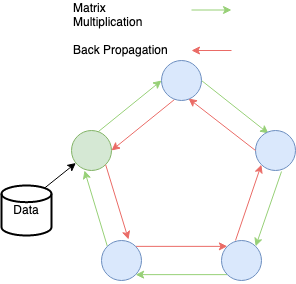
\includegraphics[width=0.3\textwidth]{ExampleNetwork}
    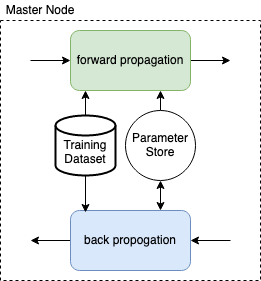
\includegraphics[width=0.3\textwidth]{masternode}
    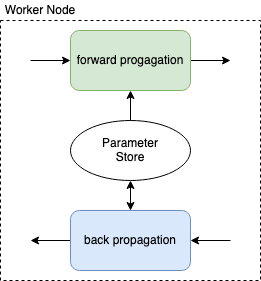
\includegraphics[width=0.3\textwidth]{SingleNode}
    \caption{
            Left: An example network of RingTMP. The green node being the master node and the blue nodes being the worker nodes.
            Centre: The architecture of the master node.
            Right: The architecture of the worker node.
        }
\end{figure}

Each batch of data follows the same path. It starts in the master node, a batch
is forward propagated through the segment of the neural network being held
locally. The intermediate result of that is send to the first worker node in the
chain. Which uses the intermediate values to forward propagated through its
neural network layers and send its results to the next node in the RingTMP
network. This continues until the last worker node in the chain makes a
prediction about the data given. This is then sent back to the master node which
calculates the loss and sends that back to the worker. The worker then uses this
to begin the backpropagation of errors back through the network. It first
updates its own parameters based on the loss. Then passes back the remaining
error back to the node before it until all the parameters have been updated.

This is different to the parameter server in several important ways. First the
model is split between the nodes, this means all thing being equal a larger
model can be trained on a RingTMP network than on a non-model parallel parameter
server. This is more of a useful feature for embedded devices where memory is at
a premium. Using the example of the EfficientNetV2-L model, which contains 121
million parameters. \cite{tan2021efficientnetv2} Estimating each of those to be
a double precision value it would amount to almost a 1 Gigabyte of data,
excluding the intermediate values stored in the RAM while performing
calculations. A non-model parallel parameter server has to be able to hold all
the variables in order for it to function, whereas in a RingTMP network the
parameters can be distributed between the layers.

Another major advantage is decreased communication between nodes. A non-model
parallel parameter server will always send more data for a
layer of the same size. This can be shown to be true thus.

The amount of arbitrary units of data sent from a parameter server to a worker
where \(n\) is the input size and \(m\) is the output size. Where \( m \geq 1\)
and \( n \geq 1\) the this can be shown to be:
\begin{equation}
    \begin{aligned}
        f(n,m) &= (n \cdot m) + m\\
        f(n,m) &= m(n+1)
    \end{aligned}
\end{equation}
The amount of arbitrary units of data sent from a RingTMP node to another node where \(m\) is
the input size and \(n\) is the output size this can be shown to be:
\begin{equation}
    g(n,m) = 2m
\end{equation}
substituting \(g(n,m)\) into \(f(n,m)\):
\begin{equation}
    \begin{aligned}
        f(n,m) &= \frac{g(n,m)}{2} \cdot (n+1)\\[1em]
        f(n,m) &= g(n,m) \cdot \frac{n+1}{2}
    \end{aligned}
\end{equation}
Given that \(n\) must be at least 1,  \( \frac{n+1}{2} \) must also be at least
1. A number multiplied by 1 or greater will always be greater than or equal to
the initial value, we can say that the parameter server will always communicate
as much or more information between nodes than RingTMP.

A simple example of this can be given to show the reduction in communication
between nodes. Take a two layer neural network the first layer having 784 input
nodes and 50 output nodes, and the second layer had 50 input nodes and 10 output
nodes. A worker sending updated weights back to a parameter server would have to
communicate 39760 values (\( (784 \times 50) + (50 \times 10) = 39860\)).
Whereas for the RingTMP model the same neural network split over two nodes would
only need to communicate 120 values. Over 300 times less network communication.

The final major advantage is the capacity for increased bandwidth between the
nodes, which built into the structure of the network. In a parameter server
model all workers connect to a single parameter server, so the network have a
star topology. This means bandwidth of the network is only as large as the
bandwidth of the parameter server, the relationship between the parameter server
bandwidth with each worker and the number of nodes in inversely proportional
(\(b = \frac{1}{x-1} where x \geq 2\)). With the RingTmp network all nodes have
two connections one ahead, one behind in a ring topology. This means no single
node will limit the bandwidth of the network. Meaning that scaling the network
will have no impact to any node if the network is physically arranged in a ring
topology.







% put equations here

% second diagram here
% second equations here

% $$a_{2} = relu(z)$$

% $$z = a_{1}w + b$$
% \begin{figure}[h]
%     \centering
%     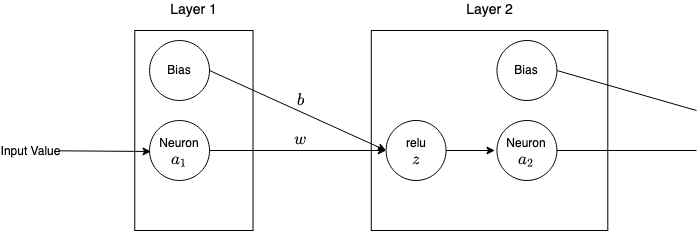
\includegraphics[width=0.6\textwidth]{simplest_neural_network_1}
% \end{figure}
% \begin{equation}
%     z_{21} = a_{11}w_{11} + a_{12}w_{12} + b_{1} \, \, \, \, \, \, \, z_{22} = a_{11}w_{21} + a_{12}w_{22} + b_{2}
% \end{equation}
% \begin{equation}
%     a_{21} = relu(z_{21}) \, \, \, \, \, \, \, a_{22} = relu(z_{22}) 
% \end{equation} 
% \begin{equation}
%     z = a_{1}w + b
% \end{equation}
% \begin{equation}
%     a_{2} = relu(z)
% \end{equation}

% The activation function being used
% in the hidden layers in this project is the ReLU function, which has become the de
% facto activation function since its discovery in 2011. \cite{glorot2011deep}
